\chapter{Actual state of the art}
\thispagestyle{pagestyle}

\section{Evolution of code editors over an entire century}
\subsection{Punch card programming}

Long before the appearance of floppy disks, magnetic tape and hard drives, programmers had an entire different way of communicating with machines. In the late 1920's, not even the first procedural languages were introduced, and the most efficient way of sending instructions to a computer back then was through so-called "punch cards".

Punch cards were designed to hold data. Such data would be stored by punching holes, which represented either letters or numbers. A character was being represented through a hole in a column. An entire line of code could be written by punching holes in about 80 bytes of rows and columns, which took an entire punch card \cite{ibm}.

Improved versions of the punch card were introduced during the following decades, but the process remained very similar, and improvements weren't as observable as they are today. Programming was still a process that required a clear and sharp mind, and couldn't be done as easily as in the present. Syntax errors in the punch card era often required the program to be rewritten from the start, as those holes couldn't be filled back.

\begin{figure}[h]
\centering
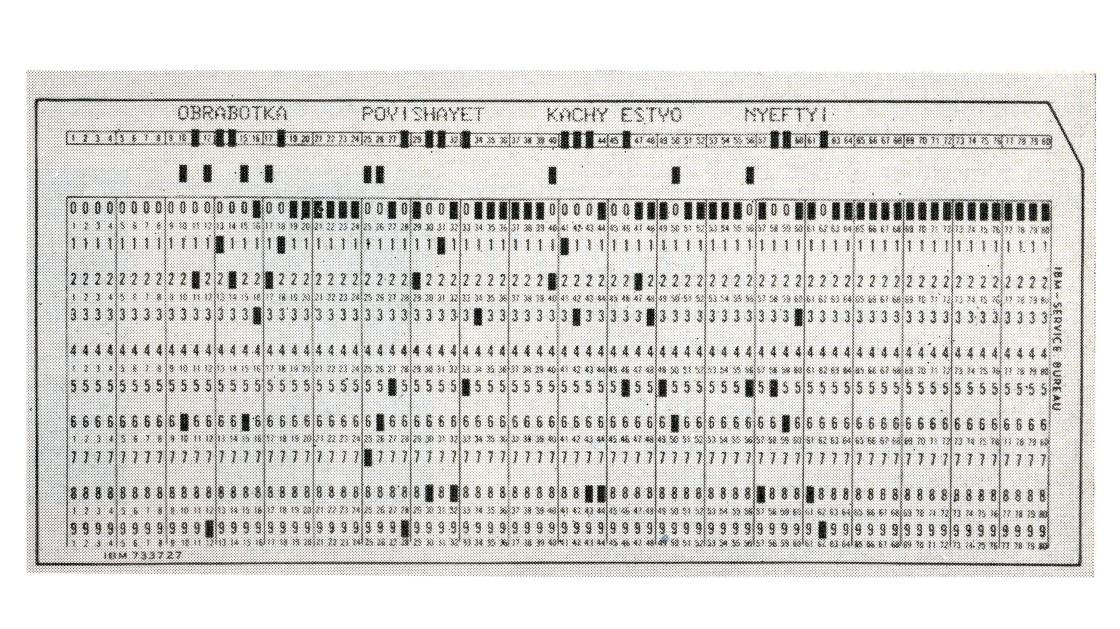
\includegraphics[width=0.5\textwidth]{images/punchcard.jpeg}
\caption{An 80-column Russian-translation punched card from 1954}
\label{fig:fig2,1.}
\end{figure}

Later, the punch card creation process was simplified thanks to the appearance of keypunch machines, which allowed code to be written using an early version of the keyboard. The machine automatically punched holes in the cards, eliminating the need for the programmer to do it manually.

\begin{figure}[h]
\centering
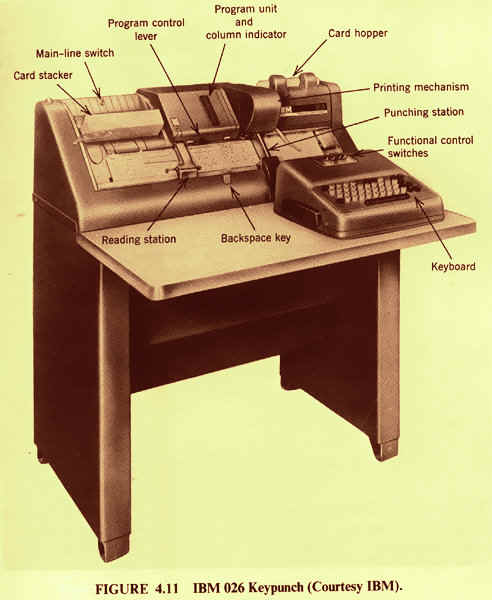
\includegraphics[width=0.5\textwidth]{images/keypunch.jpg}
\caption{The IBM 026 Key Punch}
\label{fig:fig2,1.}
\end{figure}

\subsection{First digital text editors}

A significant leap from punch cards was represented by the so-called TECO (Text Editor and Corrector), a text editor originally developed on the PDP-1 by Dan Murphy. Its release took place in 1962, more than six decades ago, and TECO is still included in some operating systems such as OpenVMS.

Even though TECO did not provide syntax highlighting and autocomplete features, it redefined the standards of text editing software by offering unique capabilities for searching and modifying text through its "macros".

In 1979, a new editor called vi entered the market. Vi was designed as a modified version of two editors written for UNIX systems: the popular ed ("editor"), which was natively integrated into UNIX, and em ("editor for mortals"). Em was a modified version of ed, created by George Coulouris.

Vi was developed by Bill Joy, a student at the time, who was dissatisfied with the capabilities of state-of-the-art editors while fixing a Pascal compiler \cite{vi}. Its ease of use and simplified user interface provided a significant advancement over TECO, which, though very powerful at the time, was considered too advanced for those who didn't want to learn all of its commands.

The introduction of mnemonic commands to manipulate text brought editors one step closer to the intuitive user interfaces we see today in modern software. However, the original vi still didn't include syntax highlighting features. A modified version of vi, called vim ("vi improved"), was released a decade later. Both editors have been included in UNIX's toolset.

\begin{figure}[h]
\centering
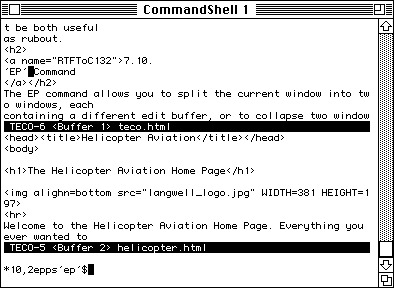
\includegraphics[width=0.5\textwidth]{images/teco.jpg}
\caption{Text Editor and Corrector (also known as TECO)}
\label{fig:fig2,1.}
\end{figure}

\begin{figure}[h]
\centering
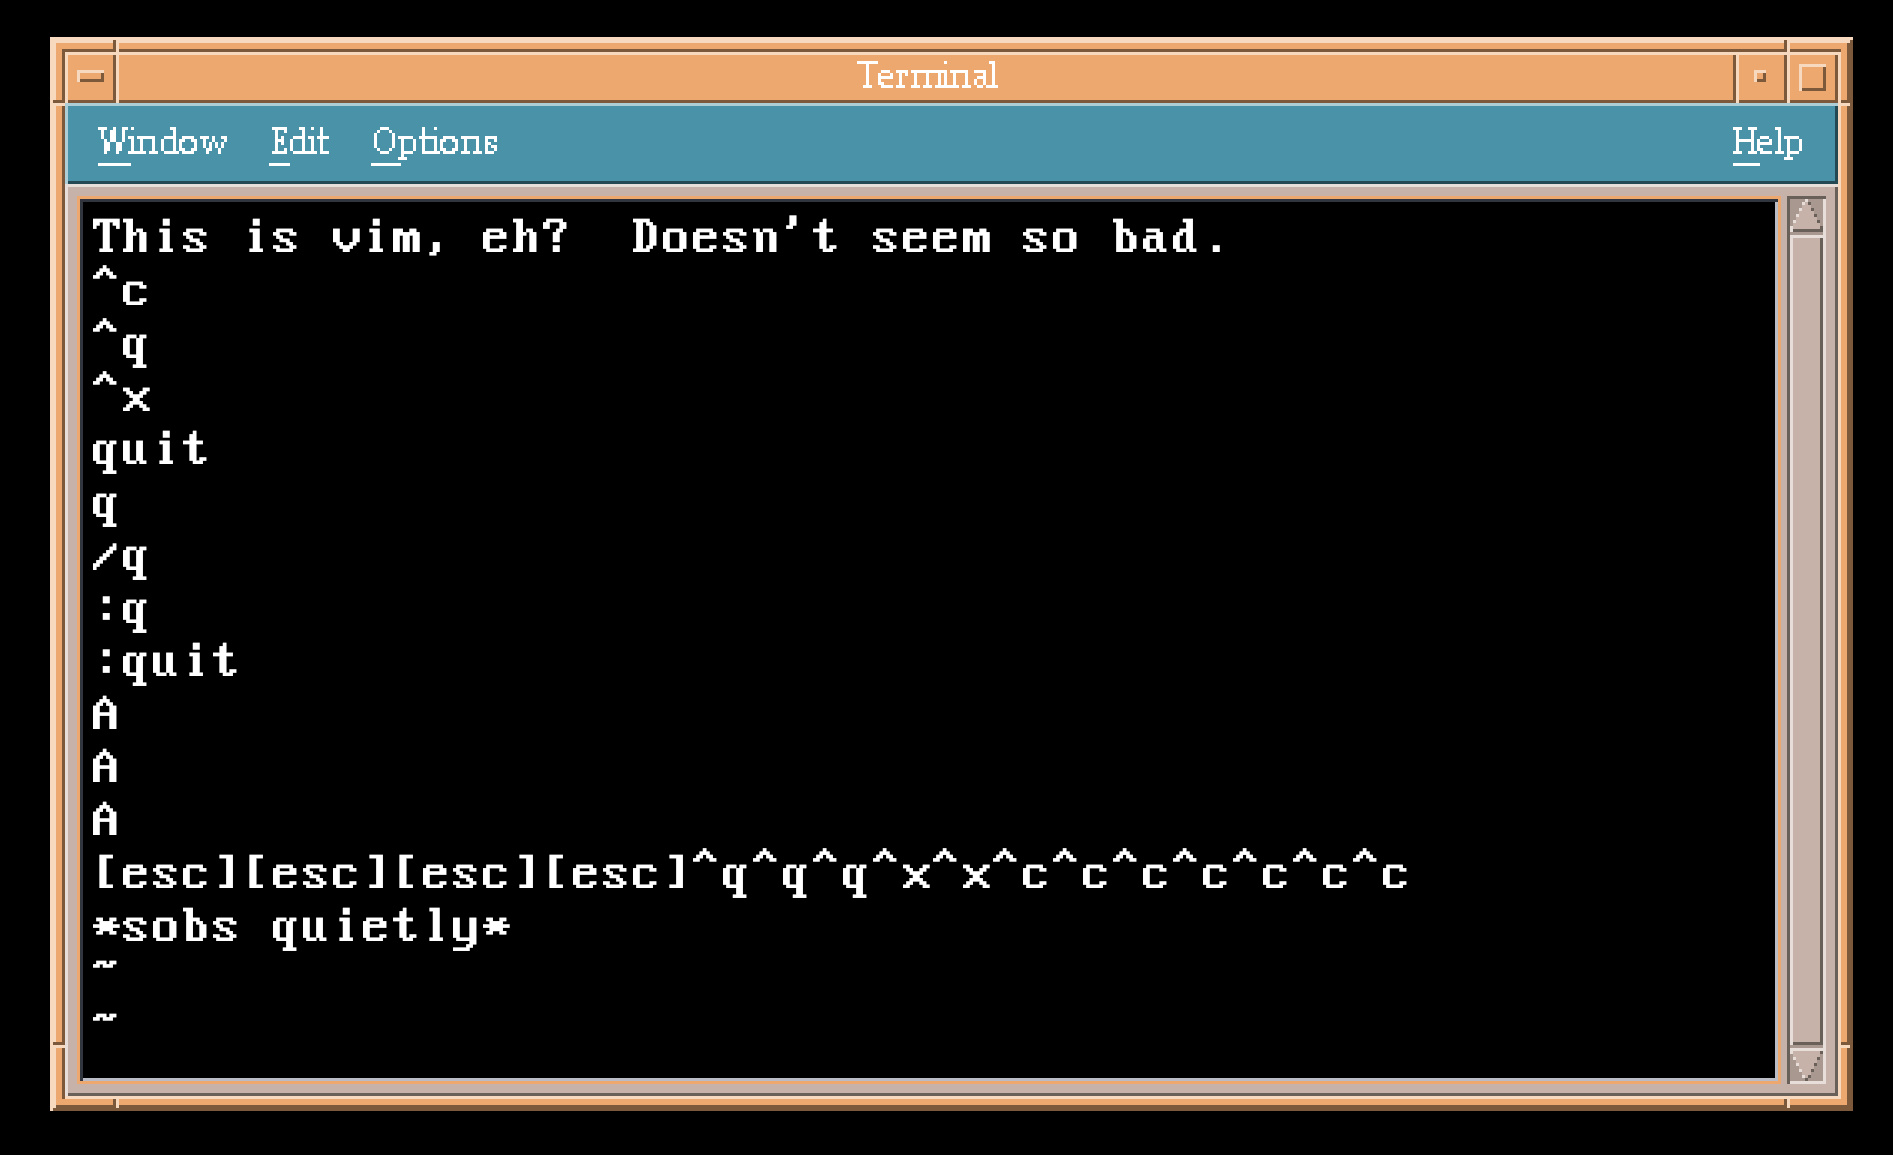
\includegraphics[width=0.5\textwidth]{images/vi.png}
\caption{vi editor}
\label{fig:fig2,1.}
\end{figure}

\subsection{Integrated Development Environments}

Several years after the release of vim, in 1991, developers realized that software projects were becoming larger and more complex than ever before. Microsoft released its first version of Visual Studio in 1997, and Eclipse launched its first open-source IDE, primarily oriented towards Java development.

Software products began to rely more on graphical user interfaces (UI), requiring intensive use of third-party dependencies and frameworks. Build tools such as Apache Ant and Maven were introduced to simplify the building process of hundreds or even thousands of files.

Terminals and command-line tools could no longer be considered acceptable media for building projects. With the release of popular frameworks such as .NET (2002), Spring (2002), and Django (2005), integrated development environments (IDEs) became the best option for software developers.

IDEs came with many features that aided the entire coding process. Refactoring, the ability to change a field's name in a class definition while automatically updating references in all of the project's files, was revolutionary at the time. Debuggers, build automation, code coverage tools, and source control management were all considered innovative and extremely helpful. Developers no longer needed to rely on external tools, as IDEs had everything packed into a single software product.

\begin{figure}[h]
\centering
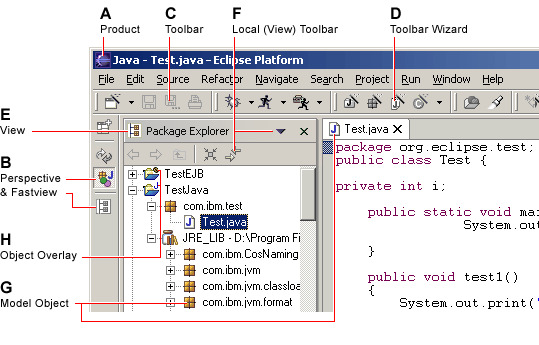
\includegraphics[width=0.5\textwidth]{images/eclipse.jpg}
\caption{Eclipse User Interface (2004)}
\label{fig:fig2,1.}
\end{figure}

\begin{figure}[h]
\centering
\includegraphics[width=0.5\textwidth]{images/visual-studio.jpg}
\caption{An actual version of Microsoft Visual Studio, featuring Drag and Drop capabilities}
\label{fig:fig2,1.}
\end{figure}

\subsection{Rise of modern code editors}

After years of continuous improvements in IDEs, it became clear that smaller projects also required a suitable medium for development. Python, although released in 1991, gained significant popularity almost 20 years later. Besides being used in frameworks such as Django and Flask, Python was also intended for scripting. Eclipse, NetBeans, and Visual Studio were not designed for projects with a smaller number of source files. While integrated development environments improved time efficiency for enterprise projects, they had the opposite effect for Python scripts or static web pages.

Text editors had already seen modern implementations, such as the release of Notepad++ in 2003, but the product was mainly intended for text formatting and manipulation, despite providing several code editing features.

Code editors, which primarily focused on assisting developers in the process of writing code rather than on the project's build process, began to be released. This started with Sublime Text (2008), and continued with the popular Visual Studio Code (2015), a lightweight, general-purpose adaptation of Visual Studio.

Nowadays, code editors are statistically the preferred option for frontend development, scripting, and small programs that can be compiled using the command line.

\begin{figure}[h]
\centering
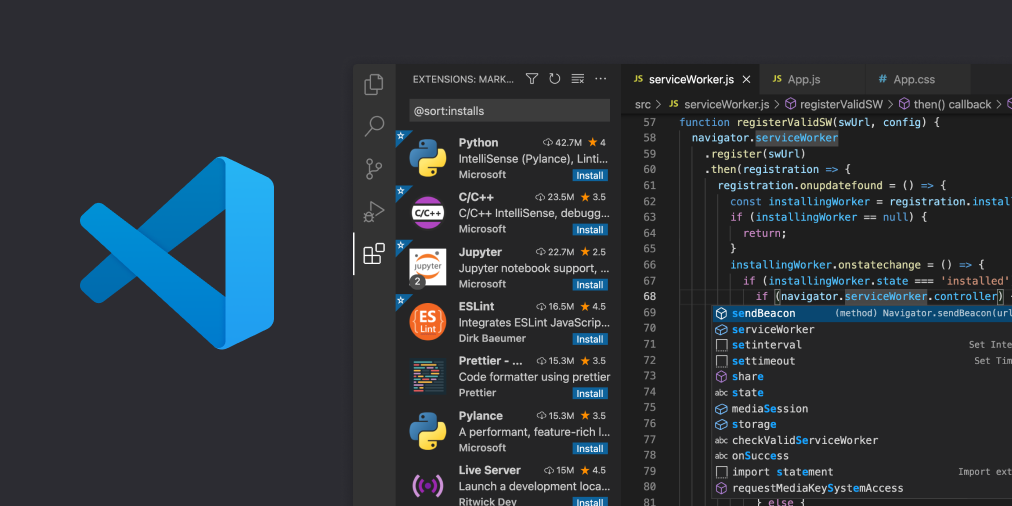
\includegraphics[width=0.7\textwidth]{images/vscode.png}
\caption{Microsoft Visual Studio Code's user interface}
\label{fig:fig2,1.}
\end{figure}

\section{Pie - An Editor Focused on Simplicity}

\subsection{The reason Pie was developed}

Smaller projects are not meant to be developed using heavyweight tools. The release of Visual Studio Code has significantly improved the process of creating small-scale applications. However, during the years, code editors such as the one mentioned before faced changes and feature additions that increased the complexity of use.

Visual Studio Code, although marketed as a tool easy to use ("Edit, build, and debug with ease" \cite{why_vscode}), bases almost its entire configuration on JSON-formatted files. Adding custom build commands (called "Tasks") requires manual editing of a tasks.json file.

\begin{lstlisting}[language=json, caption={tasks.json configuration for compiling C sources in Visual Studio Code}]
{
  "version": "2.0.0",
  "tasks": [
    {
      "label": "build",
      "command": "gcc",
      "args": ["-Wall", "helloWorld.c", "-o", "helloWorld"],
      "problemMatcher": {
        "owner": "cpp",
        "fileLocation": ["relative", "${workspaceFolder}"],
        "pattern": {
          "regexp": "^(.*):(\\d+):(\\d+):\\s+(warning|error):\\s+(.*)$",
          "file": 1,
          "line": 2,
          "column": 3,
          "severity": 4,
          "message": 5
        }
      }
    }
  ]
}
\end{lstlisting}

This code snippet is extracted from \href{https://code.visualstudio.com/docs/editor/tasks}{https://code.visualstudio.com/docs/editor/tasks}.

\hspace{0pt}

Besides from that, its language support capabilities are entirely based on extensions that need to be downloaded from an integrated download manager called "Extension Marketplace".

\begin{figure}[H]
\centering
\includegraphics[width=0.5\textwidth]{images/vscode-extensions.png}
\caption{Microsoft Visual Studio Code's "Extension Marketplace"}
\label{fig:fig2,1.}
\end{figure}

Additional settings are also very difficult to find, due to Visual Studio Code's complex user interface. Popup windows and unnecessary sidebars keep the programmer away from their main focus area - the actual code editor.

Although Visual Studio Code may seem like a good option for more complex web applications or scripts, using it on a daily basis for editing small text or source files is not what it was intended for.

Moving further to the option that may seem the best for the use cases described above, Notepad++ seems to be the editor that is capable of doing everything. It provides code support, text manipulation capabilities, and its interface is also configurable. However, many people still decide not to rely on it for their daily tasks.

Notepad++ has been released in 2003 and it hasn't updated its interface very much since then. It is oriented more towards text manipulation, as it lacks commonly used development features such as integrated terminal and version control management system. Advanced features can, indeed, be added to Notepad++, but the product requires installation of additional plugins, similar to Visual Studio Code's "extensions" system.

\begin{figure}[H]
\centering
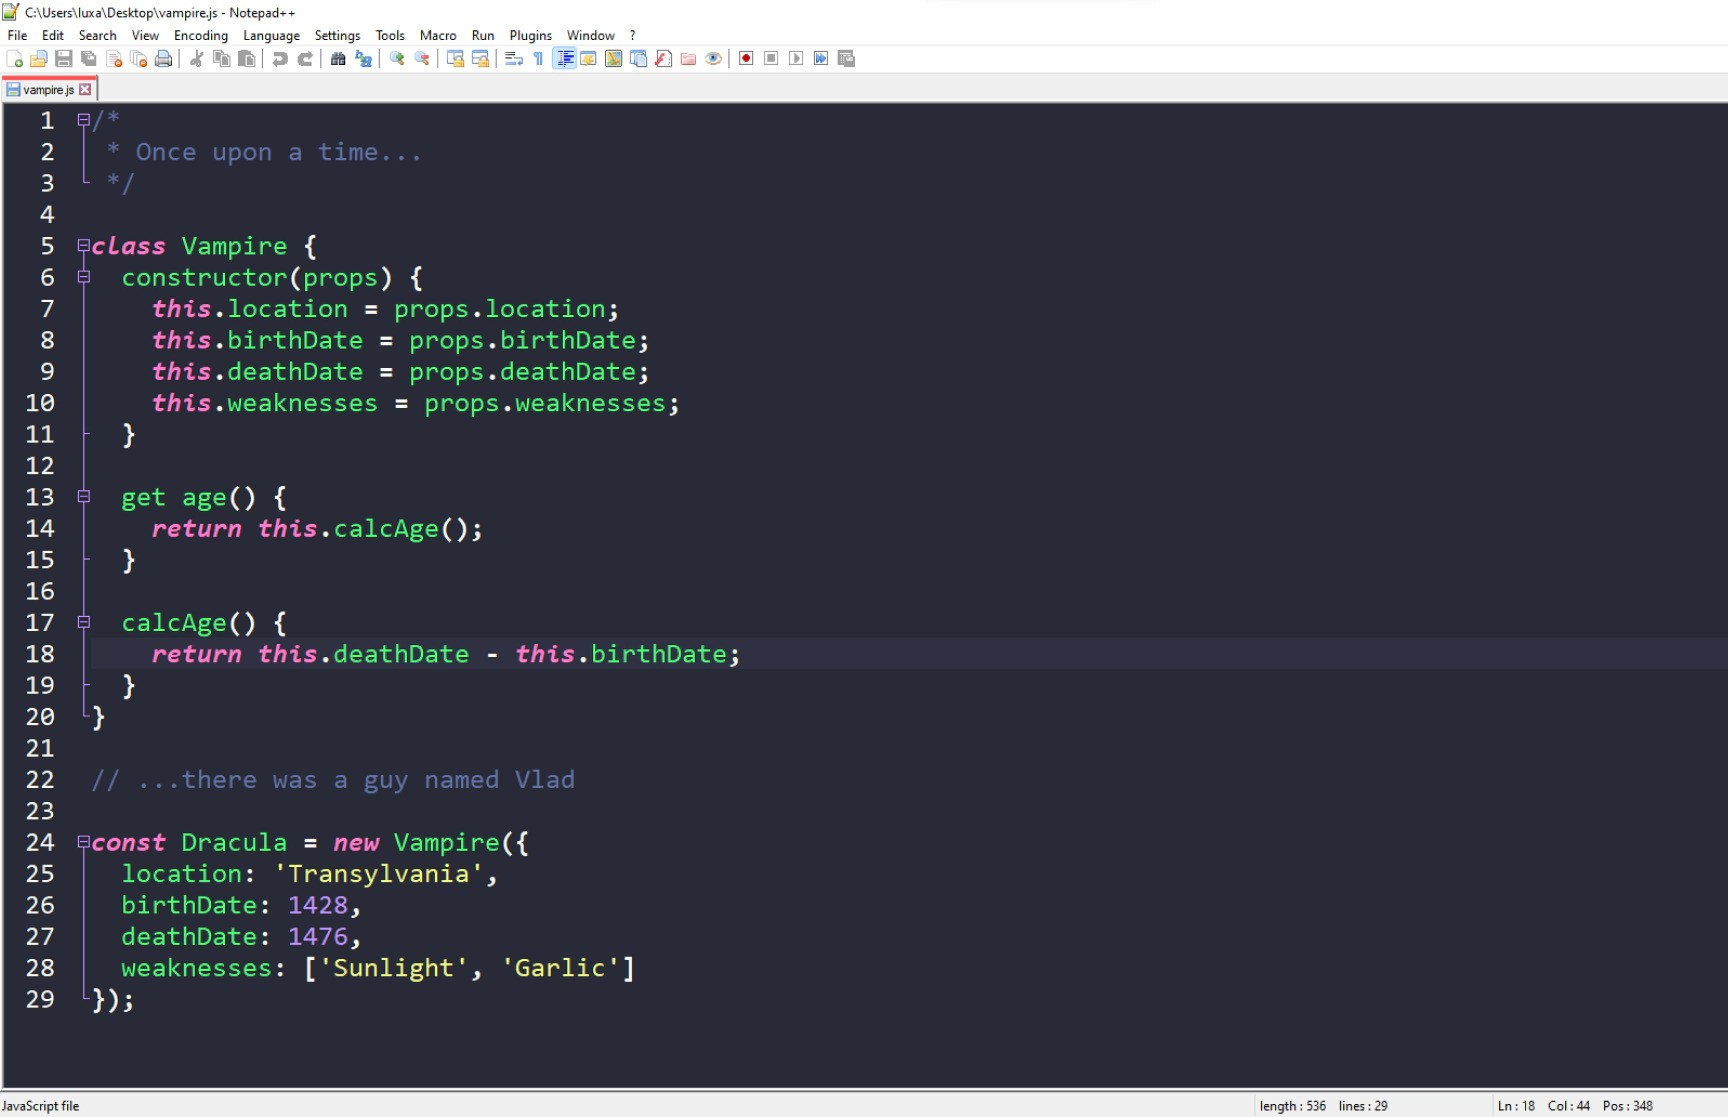
\includegraphics[width=0.8\textwidth]{images/notepad-plus-plus-dark.jpg}
\caption{Third-party "Dracula" theme for Notepad++, only changes the color of the text editor, leaving design inconsistencies}
\label{fig:fig2,1.}
\end{figure}

I have designed Pie with the purpose to fill in the lacks of Notepad++, while also keeping its user interface simple and accessible to every user. An editor made for daily use should be fast, simple and robust.

\subsection{Comparing Pie with state-of-the-art editors}

Similar to popular code editors, Pie offers syntax highlighting and code autocomplete features for various programming languages. These features are automatically toggled based on the extension of the opened file. Syntax highlighting is considered an essential feature of integrated development environments, as it has a massive impact on code comprehension \cite{syntax}.

The aspect that makes the biggest difference between Pie and potential competitors is the user interface. Pie has a user interface as clean as the classic Notepad while still offering most of what is needed for a proper development session. Compared to Notepad++ or Visual Studio Code, all of Pie's features are properly organized into categories and subcategories, making them accessible in seconds.

\begin{figure}[h]
\centering
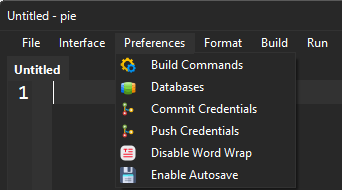
\includegraphics[width=0.5\textwidth]{images/pie-menu-strip.png}
\caption{Pie's docked menu strip, featuring the "Preferences" category}
\label{fig:fig2,1.}
\end{figure}

Pie also comes with a set of integrated development tools, such as a repository explorer for Git, a database connection manager, and integrated terminals. A vanilla version of Notepad++ doesn't provide such capabilities and requires installation and configuration of third-party plugins, which may present unexpected behavior since they are not designed by the product's original authors. Visual Studio Code offers several of these features without requiring users to navigate through their Extension Marketplace. However, because of its complex configuration model present in every aspect of the application, it requires users to spend minutes or even more to make them work as intended.

Visual Studio Code, assisted with third-party extensions, provides everything required for properly managing a database. The "Oracle Developer Tools for VS Code (SQL and PLSQL)" allows users to manipulate tables and entries the Oracle-way. However, most of these features are only required in special cases. For example, an SQL script that runs against one's database whenever a connection is established may be a good way of keeping the database secure, but it certainly isn't needed for a smaller project or for a prototype application.

\begin{figure}[h]
\centering
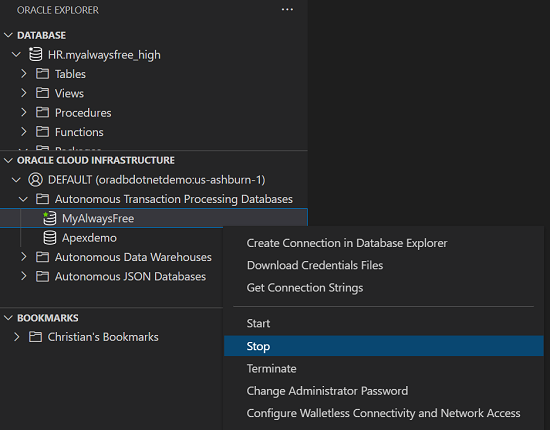
\includegraphics[width=0.6\textwidth]{images/oracledb-vscode.png}
\caption{Oracle Database connection management in Visual Studio Code}
\label{fig:fig2,1.}
\end{figure}

Pie's database connection manager is as simple as it sounds. Users add their connection details and are able to launch SQL scripts against every file with an .sql extension, directly from the context menu. No special environment needs to be opened. Whenever the user navigates through a project directory and finds an SQL file, they can directly run it against a database.

Comparing other Visual Studio Code aspects, their "Task" functionality, already mentioned in the previous subsection, allows users to input their own custom commands, which may be executed at any time. Most of the build commands are going to be executed manually by the user. Working on smaller projects won't require specifying which file patterns or directories should be built. Compared to Visual Studio Code's Tasks, Pie's "Build Commands" interface is much simpler.

\begin{figure}[H]
\centering
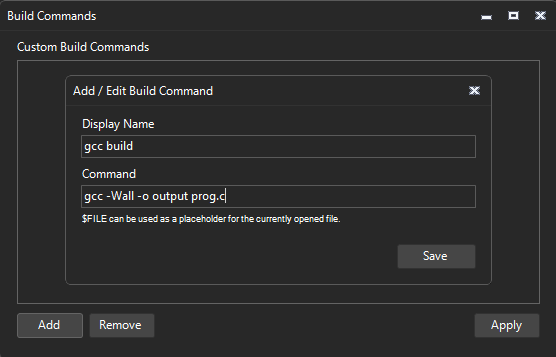
\includegraphics[width=0.6\textwidth]{images/pie-build-commands.png}
\caption{Adding a gcc build command in Pie}
\label{fig:fig2,1.}
\end{figure}

Compared to Notepad++, which is focused on text editing, Pie has several capabilities used for the same purpose. It won't be able to replace Notepad++ in special cases, where intense text manipulation is required, but its "Format" features offer most of what is required on a daily basis. Sorting a list, removing duplicate lines or lines consisting only of whitespaces are simplified ways of cleaning input or output data. Such data will be often present in software projects, no matter the size, so it was essential for them to be integrated into Pie.

The table below depicts a comparison between most popular integrated development environments or code editors and Pie. As observed, the debugging functionality is not present into Pie, because integration of specific compilers would have been required, and my product was not designed for that purpose.

\begin{table}[h]
\centering
\scalebox{0.7}{
\begin{tabular}{|*{7}{c|}}
\hline
 & \textbf{Visual Studio Code} & \textbf{Sublime Text} & \textbf{Notepad++} & \textbf{IntelliJ IDEA} & \textbf{Atom} & \textbf{Pie} \\
\hline
\textbf{Syntax Highlighting} & \checkmark & \checkmark & \checkmark & \checkmark & \checkmark & \checkmark  \\
\hline
\textbf{Autocomplete} & \checkmark & \checkmark & \checkmark & \checkmark & \checkmark & \checkmark  \\
\hline
\textbf{Automatic Indentation} & \checkmark & \checkmark & \checkmark & \checkmark & \checkmark & \checkmark  \\
\hline
\textbf{Code Folding} & \checkmark & \checkmark & \checkmark & \checkmark & \checkmark & \checkmark  \\
\hline
\textbf{Advanced Text Manipulation} & P & $ \times $ & \checkmark & P & P & \checkmark  \\
\hline
\textbf{Integrated Terminal} & \checkmark & P & P & \checkmark & P & \checkmark  \\
\hline
\textbf{Debugger} & \checkmark & P & $ \times $ & \checkmark & P & $ \times $  \\
\hline
\textbf{Custom Build Commands} & \checkmark & \checkmark & \checkmark & \checkmark & \checkmark & \checkmark  \\
\hline
\textbf{Git Integration with UI} & \checkmark & $ \times $ & $ \times $ & \checkmark & \checkmark & \checkmark  \\
\hline
\textbf{Integrated HTML Preview} & P & $ \times $ & P & \checkmark & P & \checkmark  \\
\hline
\textbf{Integrated Markdown Preview} & P & $ \times $ & P & \checkmark & P & \checkmark  \\
\hline
\textbf{Execute SQL queries} & P & P & $ \times $ & \checkmark & P & \checkmark  \\
\hline
\textbf{Customize application colors} & \checkmark & \checkmark & $ \times $ & \checkmark & \checkmark & \checkmark \\

\hline
\end{tabular}}
\vspace{2mm}
\caption{Feature comparison of popular integrated development environments, compared with Pie\\
(\checkmark - feature available, $ \times $ - feature not available, P - feature available only with installed plugin)}
\end{table}

We can now conclude the reasons Pie was developed, and why it is different from state-of-the-art IDEs:

\begin{enumerate}
  \item user interfaces in popular modern editors have become overly complex, making it difficult for new or casual users to locate essential features within the editor;
  \item integrated development environments do not emphasize commonly used features, they come with a large set of functionalities, most of them being used only in very specific cases;
  \item editors designed for daily tasks, like Notepad++, have been developed over decades but typically offer only the minimum required for software development, programmers being forced to switch between multiple apps or use additional external tools. 
\end{enumerate}

Pie is designed to be used for everything, from basic text editing and scripting, to software development, whenever it feels to much to use an integrated development environment.